\documentclass[11pt,a4paper,oneside]{report}

\usepackage{pdfpages}
\usepackage{epstopdf}
\usepackage{url}
\usepackage[toc,page]{appendix}
\usepackage{hyperref}
 \usepackage{caption}
\usepackage{subcaption}



\renewcommand{\thesection}{\arabic{section}}
\setcounter{secnumdepth}{3}

\title{\textbf{Master thesis : Fake news detection using machine learning}
\\ Review 2 Draft}

\author{Simon Lorent}

\date{Academic year 2018 - 2019}

\begin{document}
\maketitle

\section{Models}
\subsection{Model comparaison} \label{section:model_comp}

Since the last review I've introduced a few new models in addition of the Naïve-Bayes classifier. These new models are decision tree classifer, linear svm classifier and ridge classifier. I have also tried to use lasso classifier and non linear svm but these medols complexity increase too fast with respect to the sample size and thus are not possible to terminate in a reasonable amount of time. It exists libraries that run svm on GPU but I have not manage to make it works yet. In order to avoid the problem of over represation of two single domains, I've chose to discard them in the following analysis and to use them as test set. 

\begin{figure}[h]
	\centering
        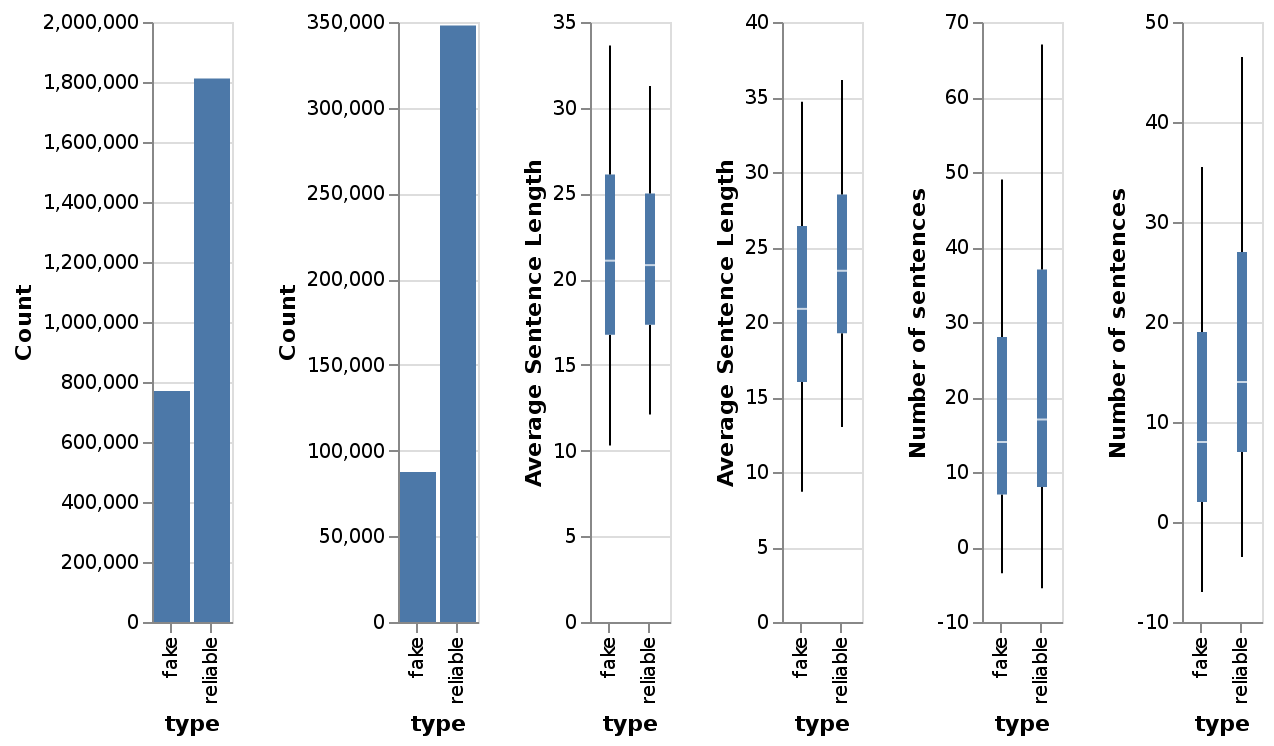
\includegraphics[width=0.8\textwidth]{output/numSentences.png}
        \caption{Summary statics on dataset, with and without downsampling.}
        \label{fig:numSentences}
\end{figure}
The linear svc shows a good improvement over the basic Naïve-Bayes. I've also try to limit the maximum number of features of the TF-IDF model and it also allows to have some improvement. This can be seen at \textbf{Figure \ref{fig:all_recall_fake}}.

\begin{figure}[h]
	\centering
	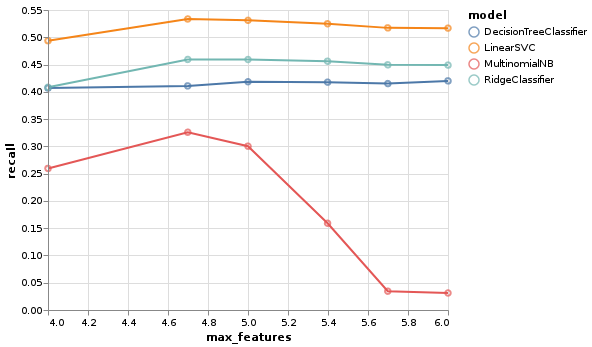
\includegraphics[width=\textwidth]{output/all_fake_recall.png}
	\caption{Model comparison with respect to the number of TF-IDF features (log scale) on fake.}
	\label{fig:all_recall_fake}
\end{figure}

\begin{figure}[h]
	\centering
	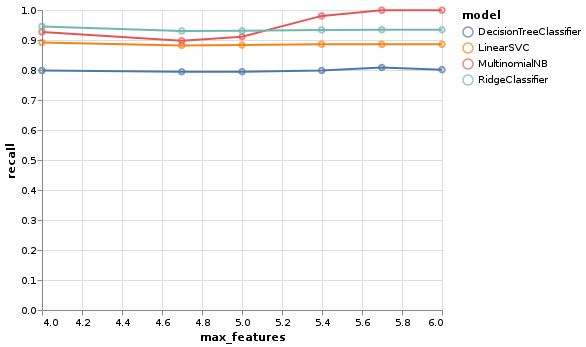
\includegraphics[width=\textwidth]{output/all_reliable_recall.png}
	\caption{Model comparison with respect to the number of TF-IDF features (log scale) on reliable.}
	\label{fig:all_recall_reliable}
\end{figure}

\begin{figure}[h]
	\centering
	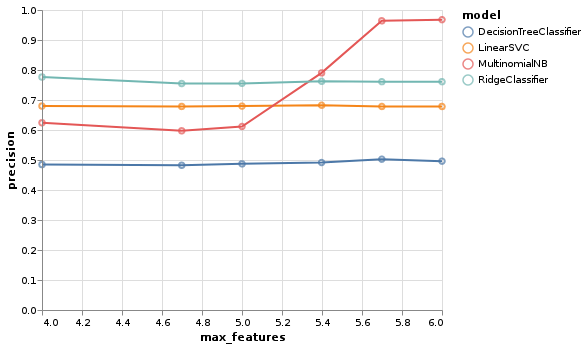
\includegraphics[width=\textwidth]{output/all_fake_precision.png}
	\caption{Model comparison with respect to the number of TF-IDF features (log scale) on fake.}
	\label{fig:all_precision_fake}
\end{figure}

\begin{figure}[h]
	\centering
	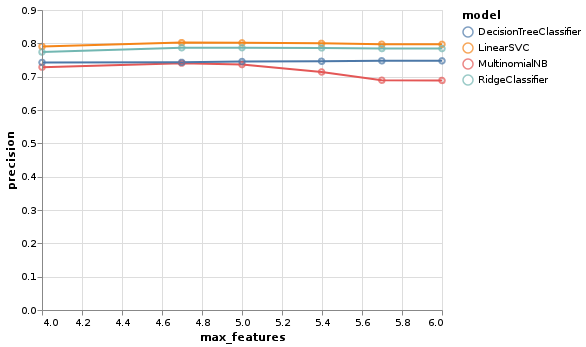
\includegraphics[width=\textwidth]{output/all_reliable_precision.png}
	\caption{Model comparison with respect to the number of TF-IDF features (log scale) on reliable.}
	\label{fig:all_precision_reliable}
\end{figure}

We can see that Naïve-Bayes has the worst recall for fake news but it is the one that perform the best on reliable news. 

\subsection{Linear SVC}
Linear SVC is a special case of SVM that fit linear model and is a lot faster than traditional SVM. \textbf{Figure \ref{fig:LinearSVC_recall}} shows the recall with respect to the paramter C, which is defined as Penalty parameter of the error term. It can be seen that this parameter does not have a lot of influence on precision or recall. It should be noted that these values are the ones of the 3-folds cross validation and not from the validation test score. See \textbf{Section \ref{section:model_comp}} for the performances on the validation set. 

\begin{figure}[h]
	\centering
	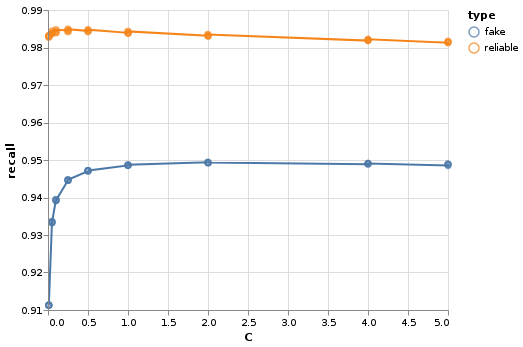
\includegraphics[width=\textwidth]{output/LinearSVC_recall.png}
	\caption{Recall with respect to the parameter C}
	\label{fig:LinearSVC_recall}
\end{figure}

\begin{figure}[h]
	\centering
	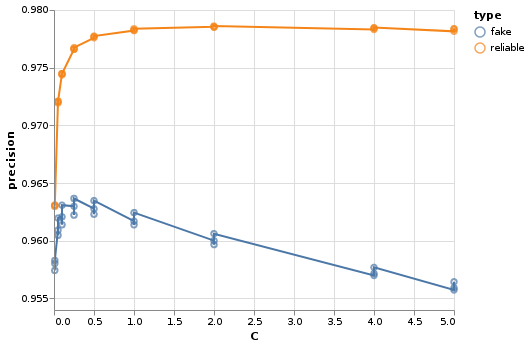
\includegraphics[width=\textwidth]{output/LinearSVC_precision.png}
	\caption{Precision with respect to the parameter C}
	\label{fig:LinearSVC_precision}
\end{figure}

\section{SMOTE}

As opposed to primilary results, SMOTE method does increase the recall for fake detection, but on the other hand is lowering the one for reliable detection, it is also lowering precision. This can be seen at \textbf{Figure \ref{fig:all_recall_fake_SMOTE}} to \textbf{\ref{fig:all_precision_reliable_SMOTE}}.

\begin{figure}[h]
	\centering
	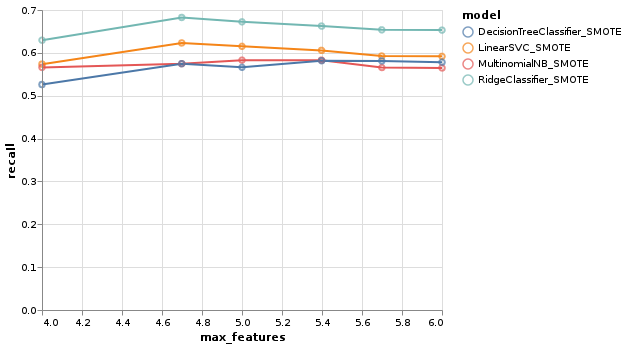
\includegraphics[width=\textwidth]{output/all_fake_recall_SMOTE.png}
	\caption{Model comparison with respect to the number of TF-IDF features (log scale) on fake.}
	\label{fig:all_recall_fake_SMOTE}
\end{figure}

\begin{figure}[h]
	\centering
	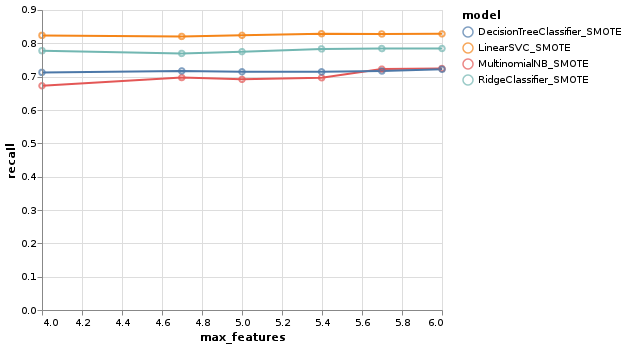
\includegraphics[width=\textwidth]{output/all_reliable_recall_SMOTE.png}
	\caption{Model comparison with respect to the number of TF-IDF features (log scale) on reliable.}
	\label{fig:all_recall_reliable_SMOTE}
\end{figure}

\begin{figure}[h]
	\centering
	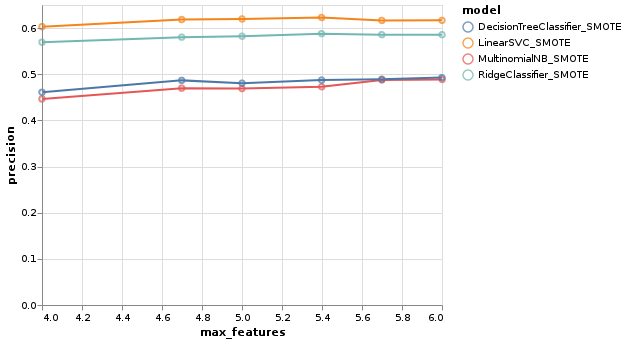
\includegraphics[width=\textwidth]{output/all_fake_precision_SMOTE.png}
	\caption{Model comparison with respect to the number of TF-IDF features (log scale) on fake.}
	\label{fig:all_precision_fake_SMOTE}
\end{figure}

\begin{figure}[h]
	\centering
	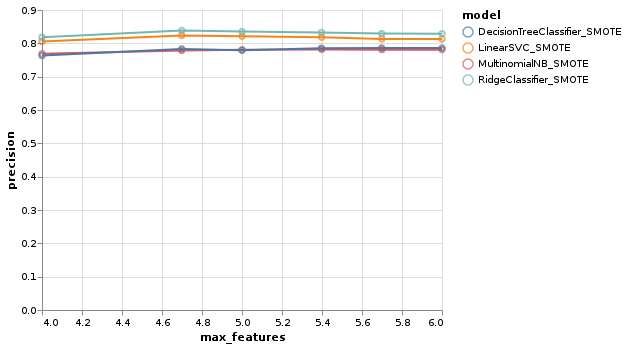
\includegraphics[width=\textwidth]{output/all_reliable_precision_SMOTE.png}
	\caption{Model comparison with respect to the number of TF-IDF features (log scale) on reliable.}
	\label{fig:all_precision_reliable_SMOTE}
\end{figure}

\section{LDA}

I have made some experiment with LDA analysis but this does not show any interesting facts, I plan to run on numerous LDA topics numbers but I need some way of mathematicaly compare the two distribution in order to find the optimal number of topics. For instance, \textbf{Figure \ref{fig:lda25}} shows the distrubtion of fake and reliable news for 25 topics and \textbf{Figure \ref{fig:lda10}} for 10 topics. 

\begin{figure}[h]
	\centering
	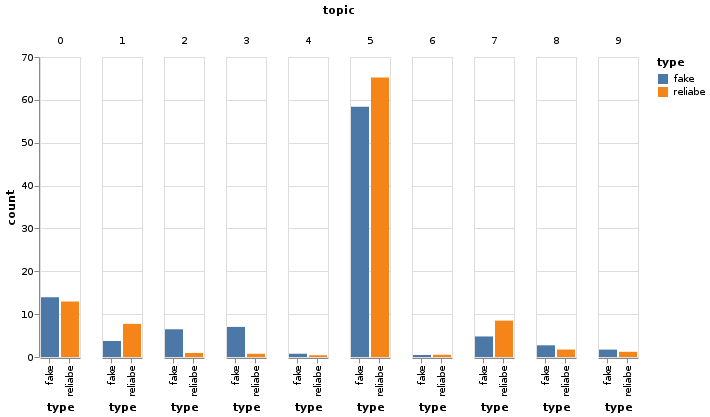
\includegraphics[width=\textwidth]{output/lda_10.png}
	\caption{News count per topics for 10 topics}
	\label{fig:lda10}
\end{figure}

\begin{figure}[h]
	\centering
	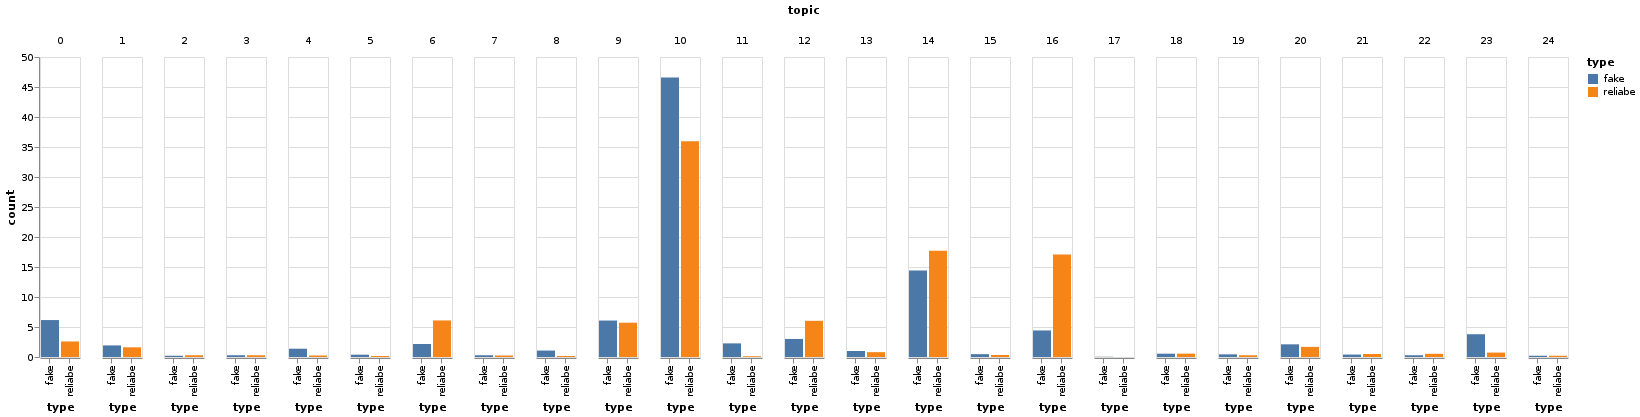
\includegraphics[width=\textwidth]{output/lda_25.png}
	\caption{News count per topics for 25 topics}
	\label{fig:lda25}
\end{figure}

\bibliographystyle{plain}
\bibliography{../references/references.bib}
\end{document}